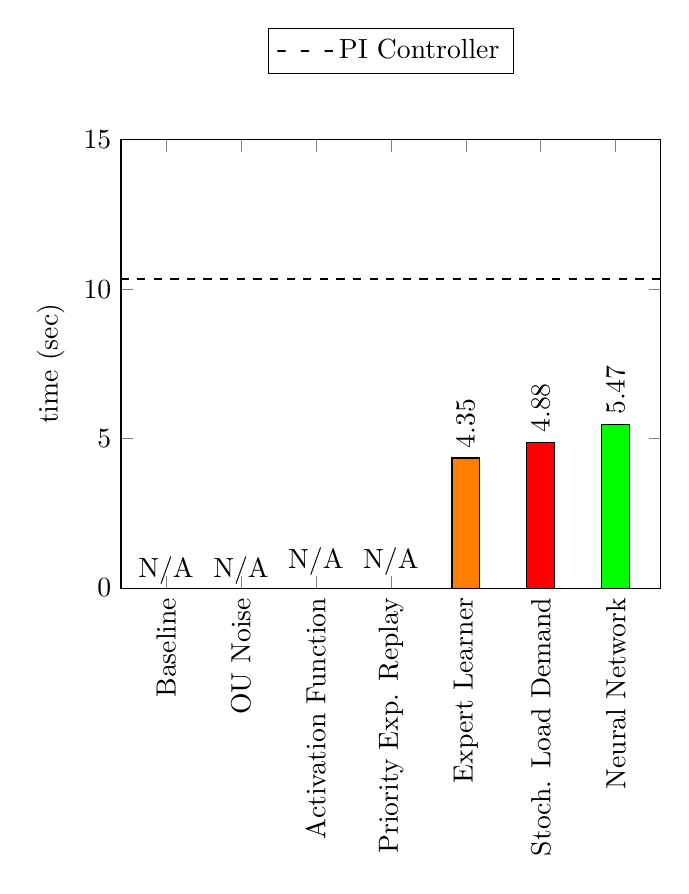
\begin{tikzpicture}
	\begin{axis}[
	    ylabel={time (sec)},
	    symbolic x coords={Baseline,, OU Noise,, Activation Function,, Priority Exp. Replay,, Expert Learner,, Stoch. Load Demand,, Neural Network},
	    xtick = {Baseline, Neural Network, Activation Function, OU Noise, Priority Exp. Replay, Expert Learner, Stoch. Load Demand},
	    xticklabel style={rotate=90},
	    nodes near coords = {%
	        \pgfmathprintnumberto[fixed,assume math mode=true]{\pgfplotspointmeta}{\myval}%
	        \pgfmathparse{\myval<0.05?:\myval}\pgfmathresult%
	    },
	    nodes near coords align={vertical},
	    every node near coord/.append style={rotate=90, anchor=west},
	    ymin=0, ymax=15,
	    legend style={at={(0.5,1.25)},anchor=north}
	    ]
	\addplot [ybar, fill=blue] coordinates {(Baseline, 0)};
	\addplot [ybar, fill=green] coordinates {(Neural Network, 5.47)};
	\addplot [ybar, fill=purple] coordinates {(Activation Function, 0)[\textcolor{red}{label}]};
	\addplot [ybar, fill=pink] coordinates {(OU Noise, 0)};
	\addplot [ybar, fill=cyan] coordinates {(Priority Exp. Replay, 0)};
	\addplot [ybar, fill=orange] coordinates {(Expert Learner, 4.35)};
	\addplot [ybar, fill=red] coordinates {(Stoch. Load Demand, 4.88)};
	%\legend{Baseline, Neural Network, Activation Function, OU Noise, Priority Experience Replay, Expert Learner, Stochastic Load Demand};
	\node at (axis cs:Baseline,0.6){\textcolor{black}{N/A}};
	\node at (axis cs:OU Noise,0.6){\textcolor{black}{N/A}};
	\node at (axis cs:Activation Function,0.9){\textcolor{black}{N/A}};
	\node at (axis cs:Priority Exp. Replay,0.9){\textcolor{black}{N/A}};
	\addplot[thick, black,dashed,sharp plot,nodes near coords={},update limits=false,shorten >=-10mm,shorten <=-10mm] 
			    coordinates {(Baseline,10.34) (Neural Network,10.34)};
	\addlegendentry{PI Controller};
	\end{axis}
\end{tikzpicture}